\documentclass[../main.tex]{subfiles}
\usepackage{silence}
\WarningFilter{glossaries}{No \printglossary or \printglossaries found}
\robExtConfigure{disable externalization}
\begin{document}
\ifSubfilesClassLoaded{%
	\graphicspath{{figures/8-Conclusions/}}%
	\setcounter{chapter}{7}%
	\mainmatter%
}{
	\graphicspath{{../figures/8-Conclusions/}}%
}
\chapter{Conclusions and Perspectives}
\minitocpage
\section{Conclusions}
	During this PhD, we explored the interest of deep learning in the field of precision medicine with a focus on omics data.
	Omics data are challenging to analyze due to their high dimensionality and the limited availability of samples.
	Our goal was to develop new deep learning methods for omics data.
	In particular, we examined the potential of the (\emph{self-})attention mechanism~\cite{AttentionAllYouNeed} to study omics data.

	In~\cref{chap:attomics}, we proposed AttOmics an architecture leveraging the self-attention mechanism to capture patient-specific feature interactions.
	To ensure the compatibility of high-dimensional molecular profiles with the self-attention memory requirements, we applied self-attention to groups of features.
	The architecture's flexibility allows the consideration of various group creation processes, particularly knowledge-based groups.
	With this approach, the number of parameters was reduced compared to an \gls{mlp} with similar dimensions while accurately predicting the type of cancer.
	Self-attention also allows the visualization of the learned interactions to understand the model better, especially when combined with knowledge-based groups.
	In our comparison with other deep learning architectures, we observed that AttOmics was the only architecture consistently performing well on different omics data.

	In~\cref{chap:crossattomics}, we proposed CrossAttOmics, a deep-learning architecture integrating multi-omics data based on the known regulatory interactions between modalities and the cross-attention mechanism.
	After encoding each modality with a modality-specific encoder, cross-attention explicitly considers interactions between pairs of modalities to build a multimodal representation.
	We extensively compared the modality combination's impact on models' performances across various architectures.
	We identified proteomics as a strong modality: selected proteins are cancer biomarkers and, therefore, good predictors.
	By using only two or three non-protein omics combinations, CrossAttOmics can achieve similar accuracy to that obtained by training only on proteins.
	CrossAttOmics outperformed other deep learning architectures when there were very few paired training examples.
	This is achieved by allowing information to flow between the different omics through the cross-attention layers.
	By explicitly modeling the interactions between different omics, attribution methods such as \gls{lrp} helped identify the most important interactions.

	In~\cref{chap:crossattomicsgate}, instead of scoring the interactions with post-hoc methods, we proposed in CrossAttOmicsGate to let the network score each interaction with a gating mechanism.
	The interaction score is used to weight the interaction embedding.
	This score is obtained by passing the cross-attention embedding of a pair of modalities to a small neural network with a single sigmoid-activated neuron.
	Gate importance scores must be sparse to ensure correct interpretability. They must also be diverse to reflect the diversity between samples, as they are patient-specific and result from complex mechanisms that differ between individuals.
	We added four regularization terms to our training process to ensure these two properties were met.
	Our ablation study showed that the four terms are essential to ensure both sparsity and diversity while improving accuracy.
	Adding interaction scores directly computed by the model during inference helps to understand how the various interactions contribute to the predictions.

	In~\cref{chap:counterfactuals}, we proposed to use \glspl{gan} to find the perturbation on the molecular profile that will change the prediction from a disease state to a healthy state.
	Those perturbations are called counterfactuals.
	The generated perturbation can help in the identification of potential biomarkers but can also provide treatment recommendations by linking the perturbation to drug databases.
	Perturbations that can change a model prediction are also known as adversarial attacks, an undesirable property of neural networks.
	To ensure our classifier's robustness and the realism of the perturbations, we compared five different adversarially trained models to identify the most robust model.

\section{Perspectives}
	This section aims to expand on the work described in this manuscript and discuss broader perspectives related to the precision medicine field.
	\subsection{Removing groups in AttOmics}\label{sec:scalar_attention}
		In \cref{chap:attomics}, we introduced AttOmics, an architecture based on the self-attention mechanism.
		To avoid self-attention limitations on high-dimensional vectors, we proposed to group features and apply the attention mechanism to these groups.
		While this approach was shown to be effective~(\cref{chap:attomics}), groups are an architectural constraint; removing them would allow for directly considering feature interactions.
		However, the self-attention operation requires elements with an embedding dimension strictly greater than one; since elements of omics profiles are scalar values with no embedding dimension, an intermediate transformation is required.
		The direct idea would be to project scalar values into a higher dimensional space and use the recent self-attention approximation~\cite{xiongNystrOmformerNystr2021,Linformer} or new efficient implementation~\cite{FlashAttention,rabeSelfattentionDoesNot2021,bolyaHydraAttentionEfficient2022a} that allows for scaling up to large inputs\footnote{see~\cite{EfficientTransformers} for an extensive overview of the possible methods}.
		Nevertheless, there is no justification for projecting scalar values into a higher space, and more importantly, it is unclear what would represent each dimension of the newly obtained vector.

		The attention matrix is obtained by measuring the similarity between pairs of inputs; for vectors, this measure is the scalar product.
		One could consider a similarity measure for scalar values, such as absolute difference, and inject this into the attention computation:
		\begin{equation}
			A_{ij} = \operatorname{softmin}\left(\left|Q_{i} - K_{j} \right| \right) \label{eq:scalar_attention}
		\end{equation}
		where \(Q_{i}\) is the \(i\)-th value in the query vector and \(K_{j}\) is the \(j\)-th value in the key vector\footnote{Note that queries, keys, and values are no longer matrices but vectors.}.
		\pythoncode[label={code:torch_att}]{Pytorch implementation of the ScalarAttention}{figures/8-Conclusions/ScalarAttentionPyTorch.py}
		This scalar formulation of the self-attention~(\cref{eq:scalar_attention}) can be easily implemented in PyTorch~(\cref{code:torch_att}) and has already been tested in~\cite{Lacan2023} but still requires to compute and store large \(d\times d\) attention matrices~(\cref{fig:lin_attention_benchA}).
		\citeauthor{Lacan2023} masked the attention matrix and only computed attention for features pairs known to be interacting (\gls{ppi})\cite{Lacan2023}.
		The \(i\)-th element of the attention output is computed as the scalar product of the \(i\)-th row of the attention matrix with the value vector.
		The \(i\)-th row of the attention matrix corresponds to the absolute difference of the query vector with the \(i\)-th value of the key vector.
		\begin{equation}
			Z_{i} = \left| Q - K_{i} \right| \cdot V
		\end{equation}
		This formulation can be implemented in an optimized triton kernel~\cite{TritonLang} as proposed in~\cref{code:triton_att}, with a lower memory footprint without significantly increasing the computation time~(\cref{fig:lin_attention_bench}).
		Triton is a programming language and a compiler to write GPU-efficient code easily.
		\pythoncode[label={code:triton_att}]{Triton implementation of the ScalarAttention}{figures/8-Conclusions/ScalarAttention.py}

		\begin{figure}[htbp]
			\centering
			\begin{subcaptiongroup}
				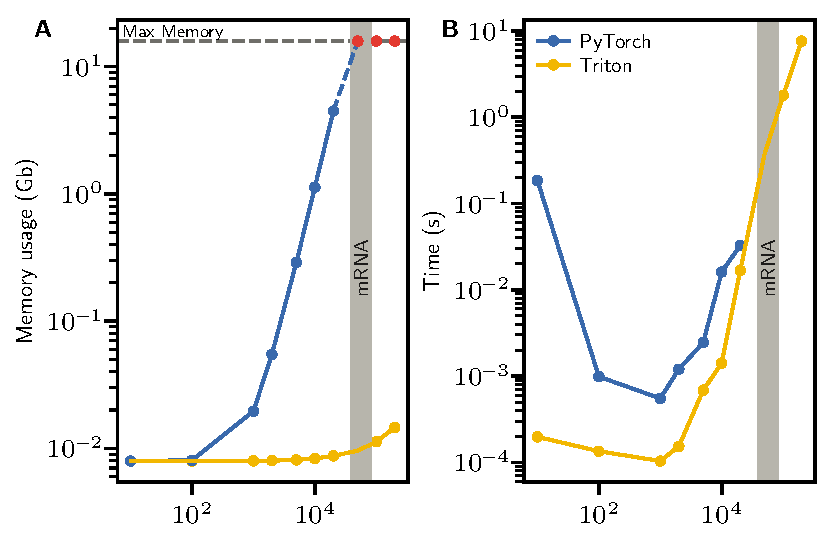
\includegraphics{ScalarAttentionBenchmark.pdf}
				\phantomcaption\label{fig:lin_attention_benchA}
				\phantomcaption\label{fig:lin_attention_benchB}
			\end{subcaptiongroup}
			\caption[Comparison of two ScalarAttention implementation]{Comparison of the memory usage~\subref{fig:lin_attention_benchA} and the computation time~\subref{fig:lin_attention_benchB} of a \textcolor[HTML]{3969AC}{PyTorch} and a \textcolor[HTML]{F2B701}{Triton} implementation of the ScalarAttention}
			\label{fig:lin_attention_bench}
		\end{figure}

	\subsection{Extending CrossAttOmics to other type of modalities}
		In \cref{chap:crossattomics}, we introduced CrossAttOmics, a deep learning architecture to integrate multi-omics data.
		As the attention mechanism can adapt any type of modalities, such as text or images, with the correct dimensions, a natural extension would be to consider non-omics modalities, such as histopathology images, clinical information, or textual reports.
		The main question would be how to connect them with the rest of the omics interactions graph~(\cref{fig:tcga_graph}).
		Furthermore, the ScalarAttention proposed in \cref{sec:scalar_attention} can be extended to multimodal context, \ie{}a CrossScalarAttention where the query comes from one modality and the key from another one.
		Such an attention mechanism would refine the considered interactions to the feature level.
		A modality interaction graph would define on which modality pairs the cross-attention is computed, and the cross-attention matrix could then be masked or regularized\footnote{see discussion on knowledge integration in \cref{sec:persp_knwoledged}.} to focus on direct relationships.
		For instance, an \gls{mirna} is expected to only interact with its \gls{mrna} targets\footnote{some \gls{mrna} targets are experimentally verified, and others are putative targets based on the sequence complementarity.}.

	\subsection{Biological knowledge}\label{sec:persp_knwoledged}
		Biolgically-informed architectures are common when applying deep learning to biological problems as they provide a strong inductive bias.
		However, adding knowledge into the deep learning architectures is challenging as they are things that are still unknown\footnote{This is probably more a philosophical question to know whether we have a complete understanding of the biological mechanism or if there is still some to be discovered.}.
		For instance, annotations mainly cover coding genes, but noncoding genes are known to be involved in gene expression regulation.
		Focusing only on annotated genes would leave out many features\footnote{For instance in \gls{go} only 14\% of the annotations involves \gls{ncrna}} and limits model capacity to consider all interactions, which at the end might limit the predictive performances.
		Moreover, excluding unannotated features prevents researchers from discovering new biomarkers that could be detected by training models on all available features.
		Instead of excluding unannotated features, a regularization favoring known relationships could be added to the training objective.
		This kind of approach allows the exploitation of knowledge while allowing the network to use unannotated features and potentially discover new feature interactions.

		Another aspect of knowledge integration is the continual construction of our understanding of biological mechanisms; some things we consider true become invalid, and newly discovered things enrich our knowledge.
		This means that a model constructed at time \(T\) might become invalid at time \(T+1\) because our knowledge has evolved.
		Models would have to be retrained to incorporate up-to-date knowledge, but constantly retraining models can be economically and environmentally costly.
		Continual learning might provide opportunities to develop AI systems that can continually acquire and update their knowledge\cite{wang2024comprehensivesurveycontinuallearning}.

	\subsection{Omics data challenges}
		Omics data are generated by different people using various methods and sequencing platforms at different places and times.
		Those variations lead to non-biological variation in the data, also known as \emph{batch effect}~\cite{Leek2010}.
		Deep learning models are sensitive to batch effects as they might capture and amplify those artifacts.
		Model interpretability can help detect such cases, but there is still a need to consider batch effects better by correcting them or adding domain adaptation tasks to ensure the same representation of all samples.
		Moreover, various tools have been developed to extract gene counts from sequencing reads, which might lead to different outputs.
		The choice of the reference genome can also impact the generated gene counts.
		It is important to ensure that all samples have been analyzed identically with fixed references.
		More initiatives, like \glsxtrshort{tcga} or ARCHS4~\cite{Lachmann2018}, are needed to provide data analyzed with a standard pipeline.

		\Gls{tcga} is an ongoing project regularly updated with new releases\footnote{\url{https://docs.gdc.cancer.gov/Data/Release_Notes/Data_Release_Notes/}} that add new data or correct erroneous information, which makes it more difficult to fairly compare various approaches since they are likely using different versions with various subset of included cancers.
		This highlights\footnote{along with the non-sharing of model weights, and in worst cases, the absence of source codes.} the need for a standardized benchmark to fairly compare multiple approaches.

		While the development of high-throughput sequencing methods increased the availability of omics data, the number of available samples remains limited compared to other deep learning fields.
		Moreover, when analyzing multi-omics data, gold standard datasets where all modalities are available for all samples are rare.
		Datasets, where some modalities are available for some patients, are more common as generating all modalities will increase the cost, or patients did not accept some analysis.
		This results in datasets with various missingness patterns where two samples have different sets of available omics.
		Such datasets are challenging to use with deep learning multimodal architectures.
		In \cref{chap:crossattomics}, we proposed to simulate the various missingness patterns during the training, which increased the robustness to missing modalities.
		Although this approach was effective, it increased the training time and supposed that all missingness patterns were generated during the training phase.
		Another way would be to generate the missing modalities from the other modalities using a generative or modality translation task.
		Generating large molecular profiles is still a difficult task as such networks are difficult to train.
		Other methods handling missing modalities project the available ones in a common latent space before combining\footnote{linear combination, product of experts, \dots} them; such models are trained in a self-supervised fashion~\cite{Lee2021AVI}.
		%TODO: Figure how to handle missing modalities 

	\subsection{Single-cell sequencing}
		This manuscript focuses on omics data obtained from bulk experiments, measuring the average expression across millions of cells.
		Current sequencing technologies allow for an increased resolution and quantify the expression at the single-cell level.
		Tumors are not composed of a single cell type; they are a mixture of various cell types harboring distinct molecular signatures~\cite{TumourHetero}.
		Using single-cell data offers new insights into the understanding of the disease and can help identify the subpopulation in the tumor susceptible to treatments~\cite{DagogoJack2017}.
		In order to apply the methods described here, datasets with paired measurements, where multiple modalities are measured from a unique cell, are required.
		While methods generating paired measurements are becoming available~\cite{Macaulay2015,Hao2021,Vandereyken2023}, they are not widely used.
		Most of the available datasets present unpaired cells, where modalities were measured on different cells.
		In addition to integrating features from different modalities, different cells need to be aligned, known as diagonal integration~\cite{Xu2022}.
		Specific integration methods are needed to solve this modality fusion problem.
		Recent technological development added a spatial dimension, giving access to the cellular organization in tissue~\cite{Vandereyken2023}.

	\subsection{Foundations models}
		Foundations models are large deep learning models trained on broad data that can be adapted to a wide range of downstream tasks~\cite{bommasani2022opportunitiesrisksfoundationmodels}.
		Large \glsxtrshort{scrna} datasets are becoming widespread: the human cell atlas~\cite{Regev2017} encompass 62 million cells.
		Such large datasets open new possibilities to train large models that can be considered foundation models~\cite{Moor2023}.
		In \citeyear{Cui2024}, \citeauthor{Cui2024} proposed scGPT a foundation model for single-cell biology~\cite{Cui2024}.
		Their model, based on a \gls{gpt} and trained on over 33 million cells, performed well in several downstream tasks after fine-tuning: cell-type annotation, multi-batch integration, genetic perturbation prediction, etc\@.
		In their architecture, self-attention was applied to the expression of each cell, \ie{}on the gene features of each cell.
		To cope with self-attention requirements, they defined a maximum number of features, 1200, randomly selected at each iteration, binned, and embedded in higher dimensional space~\cite{Cui2024}.
		Their architecture cannot handle complete expression profiles, and this limitation highlights the need for carefully designed architecture adapted to the specificity of data encountered in the biomedical field.
\end{document}
